\chapter{Measuring Beam Waist}
\label{BeamWaistAppendix}

Sometimes it's important to measure the waist of one's laser beam. This explains the exact method we use. 
  
The profile for the intensity of the beam is given by

\begin{equation} \label{electricFieldExplicitForm}
I(r,z)=I_0\left(\frac{w_0}{w(z)}\right)^2 \exp \left(\frac{-2 r^2}{w^2(z)}\right)
\end{equation}

Extrapolating this to when there are two different waists in different directions, we get: 

\begin{equation}
I(r,z)= ({\rm constants})\exp \left(-2\frac{x^2}{w_x^2(z)}-2\frac{y^2}{w_y^2(z)}\right) . 
\end{equation}

Now, total power ($P$) can be obtained by integrating the the intensity: 

\begin{align}
P&=\int_{-\infty}^{\infty}\int_{-\infty}^{\infty} ({\rm constants}) \exp \left(-2\frac{x^2}{w_x^2(z)}-2\frac{y^2}{w_y^2(z)}\right) dx dy\\
P&=\frac{\pi}{2} ({\rm constants}) w_x(z) w_y(z)
\end{align}

Now, we figure out that those constants will be

\begin{equation}
({\rm constants})=\frac{2 P}{\pi w_x(z) w_y(z)}.
\end{equation}

The ``constants'' term represents the maximum intensity that occurs within the beam (i.e. when $x=y=z=0$, or in other words, at the center of the narrowest part of the beam.)

Now, to take measurements with a knife, we block some fraction of the beam by mounting the knife on a translation stage. We then look at the amount of power from the beam hitting a photodiode that is placed downstream from the knife. If, for example, the knife is mounted vertically, the measurements on the photodiode correspond to the total power in the beam from $x=-\infty$ to $x_0$ where $x_0$ is the location of the knife. Thus, if we plot this power as a function of the spatial position of the knife, we expect that the result should be 

\begin{align}
P(x_0)&=\int_{\infty}^{\infty}\int_{-\infty}^{x_0} \frac{2 P}{\pi w_x(z) w_y(z)}\exp \left(-2\frac{x^2}{w_x^2(z)}-2\frac{y^2}{w_y^2(z)}\right) dx dy\\
P(x_0)&=\frac{P}{2} \left(\erf \frac{\sqrt{2} x}{W_x}+1 \right)
\end{align}

So, now we have a function that we can fit. The code in masterFILEhoriz14Nov.m calculates the approximate beam waist based on a series of knife cuts. First, one loads the intensity (in arbitrary units) and the position (in the units that the waist will ultimately be given in) into a number of arrays named x1, x2, .. . etc. The user types the position of the knife along the waist (show picture) into the vector called positions. 

The function d4sigma attempts to calculate the second moment width using just the raw data. This is notoriously inaccurate and also it is probably misnamed because it probably just calculates something that is different from the standard D4$\sigma$ by some factor of 2 or something. Also, we don't use this. 

Ultimately, the program does a best fit approximation to a Gaussian for each beam profile. The function we fit to is contained in the file beamWaistCalculator, which takes as its arguments the raw position data and the raw intensity data. This function is 

\begin{equation}
f(x)=a_1 \erf \left(\frac{x-a_3}{a_2}\right)+a_4.
\end{equation}

beamWaistCalculator thus returns a vector containing $(a_1 a_2 a_3 a_4)$. Thus, to get the beam waist, we will take $a_2$ and multiply by $\sqrt{2}$. 

According to Siegman \cite{SiegmanBeamQuality}, the second moment width always propagates according to this equation: 

\begin{equation}
W_x^2(z)=W_{0x}^2 + M_x^4 \left( \frac{\lambda}{\pi W_{0x}}\right)^2 (z-z_{0x})^2. 
\end{equation}
Of course, for a Gaussian beam, we recognize that allowing $M_x^2\rightarrow 1$ gives us the equation for how the waist changes as it propagates. 

This function then tries to fit to this:
\begin{equation}
W_x=a_1 \sqrt{1+\left(\frac{(x-a_2) \lambda}{\pi a_1^2}\right)^2}
\end{equation}
and this:
\begin{equation}
W_x=a_1 \sqrt{1+(1+a_3^2) \left(\frac{(x-a_2) \lambda}{\pi a_1^2}\right)^2}. 
\end{equation}
The first case we are forcing $M^2$ to be one. This gives us a worst-case scenario. A few test cases convinced us that if $M^2$ is higher than we think it is, we have a less-tightly focused center. Thus, for the purposes of not putting too much power into the AOM, we go with the fit to the first equation. 

In principle, we should be able to fit the calculated second moment widths to the equations above, but they don't work overly well. Thus, we usually use the second moment width of the Gaussian we fit it to. 

Using this method, we have determined the waist to be 


\section{Using the camera}
We initially wanted to measure the $M^2$ of our beam. The measurements are hard to do accurately. We tried to use the camera and got results that were not entirely usable.

\subsection{Investigation of feasibility of using the camera}

The camera seems like an appealing device to use to measure beam parameters since it can take large amounts of 2D data quickly.

%insert plot of pixel count vs whatever? eh, maybe.

To investigate the camera's feasibility, we wanted to verify that the camera was (a) linear and (b) that each pixel reading was independent of the rest of the image. To this end, we took several images of the same beam, which we attenuated using the polarizing beam cube/waveplates adjustable attenuator setup described in Appendix\,\ref{twoWaveplateTrick}. We took 20 measurements. Each time we measured the total intensity of the beam using a photodiode and we took a corresponding image of the beam

\begin{figure}
\centerline{
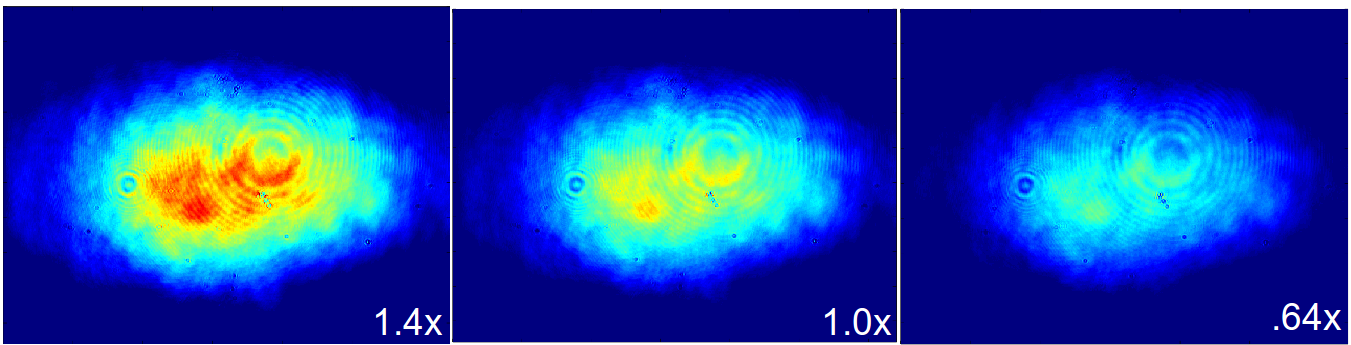
\includegraphics[width=0.95\textwidth]{cameraimage}
}
\caption[Sample Images]{Three images taken using the camera. Each was the same laser beam with the attenuation adjusted using our waveplate and polarizer setup. The total power was measured using a photodiode and the relative total power is shown in the lower right corner of each image. By comparing the pixel values of similar spots within the image, we were able to bootstrap some calibration parameters for the camera.}
\end{figure}

Our idea was that, if the camera is linear and the pixels act independently, the following statements should be true: 
\begin{itemize}
\item The ratio of the reading on any pixel to the reading on the same pixel in a different image should be equal to the ratio of the total power of the two beams used in the two readings as measured by the photodiode. 
\item Any two pixels reporting the same number of counts are experiencing the same radiance.
\end{itemize}

Thus, for example, if we see that the pixel located at $(214,442)$ has a pixel count of 127 in image 15, on which we measured the intensity to be proportional to 85.350, then we assume that we can compare it directly to a pixel located at the same location $(214,442)$ on image 20 (which had an intensity proportional to 119.70). If the reading from the $(214,442)$ pixel on image 20 was 155.46, we assume that a pixel count of 155.46 corresponds to $119.70/85.350=1.4025$ times as much intensity as a pixel count of 127. Additionally, we assume that any pixel we find in any of the images that reports a reading of 155.45 will have the same intensity as any other. 

We went through the 20 images like this: We selected some reference pixel. We then added that pixel to a master list. We then found the corresponding pixels in the other images whose position on the grid match that of the reference pixel. They were then added to the master list, making note of their position, the reading on the pixel (count) and the assumed ratio between the amount of light hitting that pixel and the amount of light hitting reference pixel as inferred based on the readings from the photodiode.

Then, we select a random pixel from the master list and look for other pixels that have the same number of counts within any of the images. If a pixel has the same reading (number of counts) as the randomly selected pixel in the master list, it is added to the master list. Since this new pixel has the same counts as the randomly selectd pixel, we assume that the pixels have the same radiance relative to the reference pixel. Once the new pixel is added to the maseter list, we find the corresponding pixels from the other images and add them to our list. We assume that the true irradiance at these pixels is proportional to the irradiance of pixel we just added. 

In this way, we create a very long list of pixels, their counts and what we have inferred about the incident illumination of each pixel by comparing it to (a) other pixels that read the same value and (b) pixels in other images of different intensities. Note that the pixels in the list are not unique. Pixels can appear multiple times in the list.

If we plot the expected pixel count (as calculated by taking the reading on the main reference pixel and multiplying it by the relative radiance factors that we've been tracking) vs the actual pixel count, we get the plot in Fig.\,\ref{cameraPixelFit}, which seems to validate the assumption of pixel independence.

However, as one can see, the camera actually has a minimumt threshold below which it does not report light very well. Because the camera throws away information and has a minimum intensity threshold to register, we throw out any $M_{i j}=0$. This way our function doesn't get penalized for showing a non-zero intensity for pixels that read out zero. The number of $M_{i j}=0$ obviously doesn't change as we try different iterations of $f(M_{ij})$, so there's no way to game our little metric to make it not work.
%We did a standard fit to a 4th order polynomial and got a reasonable function to correct for the pixel values. We were a little worried about bias in the selection of pixels and things like that. We wasted some time trying to figure out how to do this better. 

We performed a curve fit to model our pixels response. In order to do this, we had to devise a cost function that produces some figure of merit to tell us whether our test function is succeeding at making all of the pixels have the right ratio. The way it works is this: Suppose that $M_{i j}$ is a big list of our pixels. $j$ runs from 1 to 20, corresponding to the 20 different images. $i$ represents all the pixels in our image\footnote{Thus, if we are analyzing 8x8 bins, we should have 480/8*640/8=4800 pixels and i will range between 1 to 4800}. Let $f(p)$ be the proposed function that takes as its argument the count on a given pixel and gives as its output something that scales with the actual intensity of the light. The figure of merit that we can use to optimize $f(p)$ is calculated as follows: 

\begin{equation}\label{fom}
{\rm Figure\:of\:merit}=\sum_{ M_{i j}\neq 0}\left(\frac{f(M_{i j})/P_j}{{\rm average\,of\,all\,nonzero\,} f(M_{i j})/P_j {\rm \,for\,the\,ith\,pixels}}-1\right)^2
\end{equation}

where $P_j$ is the power of the jth image.

In words, Eq.\,\ref{fom} can be described as follows: First, act on the pixels with the proposed function. Then, scale them according to the intensity ratios (i.e. the ith pixel in image 1 gets divided by $P_1$ while the ith pixel in image 3 gets divided by $P_3$). Then, see by what fraction the intensity of that pixel differs from the average of the intensities calculated using data from the pixels corresponding to that one. If the function really were to find the ratio perfectly, then $f(M_{ij})/P_j$ should be exactly the same for the ith pixel from each of the j images. 


We used this function to calculate what correction function to use. We did a couple of them and found great agreement with the inversion of the previous function--thus suggesting that our previous method was acceptable. 


\begin{figure}
\centerline{
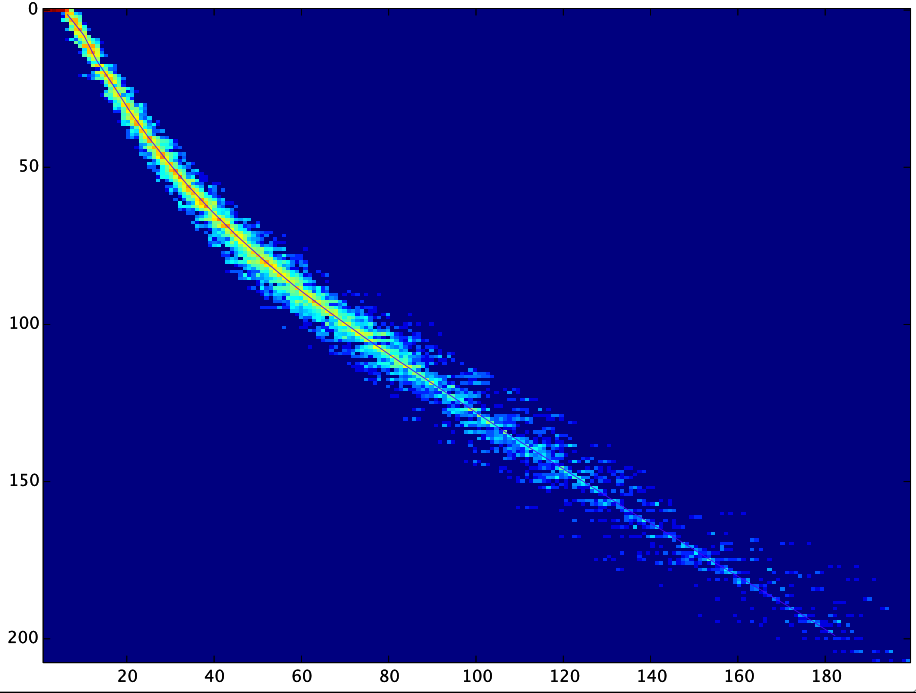
\includegraphics[width=0.95\textwidth]{cameraPixelFit}
}
\caption[Camera Linearity and Offset]{On the x axis is the inferred pixel reading based on our assumptions about the ratios of pixel readings. On the y axis, we can see the actual readings of the pixels. This illustrates clearly the threshold issue of the camera.}
\end{figure}

In the end, the camera offset and nonlinearity made it unsuitable for sensitive measurements of the second moment width of the beam. However they did provide a reasonable sanity check on our methods.
%\end{document}
